% !TEX encoding = UTF-8
% !TEX TS-program = pdflatex
% !TEX root = ../tesi.tex

%**************************************************************
\chapter{Verifica e validazione}
\label{cap:verifica-validazione}
%**************************************************************


\section{Accessibilità}
\subsection{Elementi di accessibilità}
Per rendere la navigazione al sito accessibile da tutte le categorie di utenti sono stati fatti alcuni accorgimenti:
\begin{itemize}
    \item sono presenti gli attributi \textit{accesskey} con chiave uguale alla prima lettera della parola del \textit{tag label} associato, in modo da migliorare l'accessibilità alle \textit{form} da tastiera senza l'uso del \textit{mouse};
    \item tutte le immagini contengono i \textit{tag alt}, che sono stati lasciati vuoti nel caso servissero solo per il \textit{layout};
    \item è presente una barra di navigazione che aiuta a navigare nel sito;
    \item i \textit{form} contengono dei \textit{tag label} per ogni \textit{input}, tuttavia non sono stati aggiunti \textit{tag optgroup} o \textit{fieldset} in quanto sono utili nel caso di \textit{form} molto grandi, ma essendo presenti solo \textit{form} di piccole dimensioni è stato ritenuto non necessario;
    \item sono presenti degli aiuti contestuali che mostrano gli errori nel caso fossero presenti;
    \item è presente del testo nascosto utile agli utenti con disabilità visive, come il \textit{link} con la funzione  di saltare al contenuto, ovvero di permettere di non far leggere allo \gls{screen reader} la barra di navigazione, passando direttamente al contenuto, ed è presente all'inizio della navigazione per segnalare che le scorciatoie da tastiera sono attive;
    \item sono stati evitati testi scorrevoli, lampeggianti, barrati ed in generale \textit{font} troppo elaborati per agevolare la lettura.
\end{itemize}

\section{Verifica del GruppiService}
In parallelo con la fase di codifica del \gls{microservizio} \nameref{par:GruppiService} è stata verificata la correttezza delle funzioni presenti nella classe \texttt{GruppiController}. \\
Sono stati effettuati dei test di unità utilizzando \textbf{JUnit} e \textbf{Mockito}, \gls{framework} di \textit{testing} per il linguaggio Java.\\
Per avere una reportistica dei test effettuati è stato utilizzato \textbf{JaCoCo}, strumento che fornisce informazioni sulla \textit{lines coverage}, \textit{branches coverage} e \textit{cyclomatic complexity}. 
L'attività di verifica si è rivelata molto proficua, permettendomi di agevolare lo sviluppo in modo significativo, tanto da produrre un
grande quantitativo di test, con un elevata copertura di casistiche, garantendo così qualità del prodotto.\\
Come dimostra la \textit{code coverage} (figura \ref{img:code-coverage}) è stata raggiunta la massima copertura del codice, senza che questo inficiasse sulle tempistiche programmate.

\begin{figure}[H] 
    \centerline{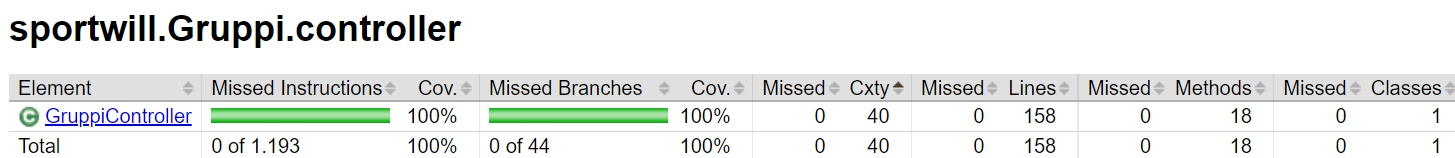
\includegraphics[scale=0.3]{verifica/coverage-gruppi-controller.jpg}} 
    \caption{Code coverage della classe \texttt{GruppiController}}
    \label{img:code-coverage}
\end{figure}

\subsection{Test effettuati}

\begin{center}
  {\rowcolors{2}{color1}{color2}	    % rows height
    \renewcommand{\arraystretch}{1.60}
    \begin{longtable}{
      |>{\centering\arraybackslash}p{48pt}
      |>{\centering\arraybackslash}p{308pt}
      |>{\centering\arraybackslash}p{27pt}|}

      \rowcolor{antimaincolor!0}
      \caption{\label{tab:Test di unita}Test di unità}

      \\

      \hline
      % header
      \rowcolor{maincolor}
      % header color
      \color{antimaincolor}{Codice}
                  &
      \color{antimaincolor}{Descrizione}
                  &

      \color{antimaincolor}{Esito}

      \\
      \hline
      \endhead

      \hline
      % header
      \rowcolor{maincolor}
      % header color
      \color{antimaincolor}{Codice}
                  &
      \color{antimaincolor}{Descrizione}
                  &

      \color{antimaincolor}{Esito}

      \\
      \hline
      \endfoot

      TU1
                  & Il metodo \texttt{getAllGruppi}
      deve restituire tutti i gruppi presenti

                  & S                                              \\
      TU2
                  & Il metodo \texttt{getAllGruppi}
      deve restituire un \texttt{HttpStatus.NO\_CONTENT} nel caso non siano
      presenti
      gruppi
                  & S                                              \\
      TU3
                  & il metodo \texttt{getGruppo} deve
      restituire il gruppo specificato nel caso sia presente
                  & S                                              \\
      TU4
                  & il metodo \texttt{getGruppo} deve
      restituire un \texttt{HttpStatus.NO\_CONTENT} nel caso non sia presente
      il
      gruppo
                  & S                                              \\
      TU5
                  & Il metodo
      \texttt{getUtentiByGruppo} deve restituire gli utenti di un gruppo
                  & S                                              \\
      TU6
                  & il metodo \texttt{createGruppo}
      deve creare un gruppo
                  & S                                              \\
      TU7
                  & Il metodo \texttt{createGruppo}
      deve restituire un \texttt{ HttpStatus.BAD\_REQUEST} nel caso non esista
      il
      proprietario del gruppo specificato
                  & S                                              \\
      TU8
                  & Il metodo \texttt{createGruppo}
      deve restituire un \texttt{ HttpStatus.BAD\_REQUEST} nel caso che le
      coordinate
      geografiche inserite non siano valide
                  & S                                              \\
      TU9
                  & Il metodo \texttt{modifyGruppo}
      deve modificare un gruppo
                  & S                                              \\
      TU10
                  & Il metodo \texttt{modifyGruppo}
      deve restituire un \texttt{ HttpStatus.NOT\_MODIFIED} nel caso il gruppo
      specificato non esiste
                  & S                                              \\
      TU11
                  & Il metodo \texttt{modifyGruppo}
      deve restituire un \texttt{ HttpStatus.BAD\_REQUEST} nel caso non esista
      il
      proprietario del gruppo specificato
                  & S                                              \\
      TU12
                  & Il metodo \texttt{deleteGruppo}
      deve eliminare un gruppo
                  & S                                              \\
      TU13
                  & Il metodo \texttt{deleteGruppo}
      deve deve restituire un \texttt{ HttpStatus.BAD\_REQUEST} nel caso non
      esista
      il gruppo specificato
                  & S                                              \\
      TU14
                  & Il metodo
      \texttt{getUsciteByGruppo} deve restituire le uscite di un gruppo
                  & S                                              \\
      TU15
                  & Il metodo
      \texttt{getUsciteByGruppo} deve restituire un \texttt{
        HttpStatus.BAD\_REQUEST}
      nel caso non esista il gruppo specificato
                  & S                                              \\
      TU16
                  & Il metodo
      \texttt{getGruppiOfUtente} deve restituire i gruppi a cui partecipa un
      utente
                  & S                                              \\
      TU17
                  & Il metodo
      \texttt{addUtenteToGruppo} deve aggiungere un utente ad un gruppo
                  & S                                              \\
      TU18
                  & Il metodo
      \texttt{addUtenteToGruppo} non deve aggiungere un nuovo utente nel caso
      il
      gruppo abbia superato il numero massimo di utenti
                  & S                                              \\
      TU19
                  & Il metodo
      \texttt{addUtenteToGruppo} deve restituire un \texttt{
        HttpStatus.BAD\_REQUEST}
      nel caso non esista il gruppo specificato
                  & S                                              \\
      TU20
                  & Il metodo
      \texttt{removeUtenteFromGruppo} deve rimuovere un utente da un gruppo
                  & S                                              \\
      TU21
                  & Il metodo
      \texttt{removeUtenteFromGruppo} deve restituire un \texttt{
        HttpStatus.BAD\_REQUEST} nel caso non esista il gruppo specificato
                  & S                                              \\
      TU22
                  & Il metodo
      \texttt{deleteUtenteFromJointUtenteCrew} deve rimuovere un utente dalla
      tabella
      \texttt{joint\_utenti\_crew}
                  & S                                              \\
      TU23
                  & Il metodo
      \texttt{addUscitaToGruppoCrew} deve aggiungere un'uscita ad un gruppo
                  & S                                              \\
      TU24
                  & Il metodo
      \texttt{addUscitaToGruppoCrew}	deve restituire un
      \texttt{HttpStatus.BAD\_REQUEST} nel caso non esista l'uscita specificata
                  &
      S
      \\
      TU25
                  & Il metodo
      \texttt{addUscitaToGruppoCrew} deve restituire un
      \texttt{HttpStatus.BAD\_REQUEST} nel caso non esista il gruppo
      specificato &
      S
      \\
      TU26
                  & Il metodo
      \texttt{removeUscitaFromGruppo} deve rimuovere un'uscita dal gruppo
      specificato
                  & S                                              \\
      TU27
                  & Il metodo \texttt{removeUscitaFromGruppo} deve
      restituire un \texttt{HttpStatus.BAD\_REQUEST} nel caso non esista
      l'uscita
      specificata
                  & S                                              \\
      TU28
                  & Il metodo \texttt{removeUscitaFromGruppo} deve
      restituire un \texttt{HttpStatus.BAD\_REQUEST} nel caso non esista il
      gruppo
      specificato
                  & S                                              \\
      TU29
                  & Il metodo
      \texttt{deleteUscitaFromJointUscitaCrew} deve rimuovere un'uscita dal
      gruppo
      specificato
                  & S                                              \\
      TU30
                  & Il metodo
      \texttt{deleteUscitaFromJointUscitaCrew} deve restituire un
      \texttt{HttpStatus.BAD\_REQUEST} nel caso non esista l'uscita specificata
                  & S
      \\
      TU31
                  & Il metodo
      \texttt{deleteUscitaFromJointUscitaCrew} deve restituire un
      \texttt{HttpStatus.BAD\_REQUEST} nel caso non esista il gruppo
      specificato &
      S
      \\

    \end{longtable}
  }
\end{center}





% \section{Validazione e collaudo}



